\documentclass[12pt]{article}

% packages :
\usepackage[utf8x]{inputenc}
\usepackage[T1]{fontenc}
%\usepackage[francais]{babel}
%
\usepackage{graphicx} % images
\usepackage{float}
\usepackage{placeins}
\usepackage{multirow}
\usepackage{wrapfig}
\usepackage{array}

% to draw circuits
\usepackage{siunitx}
\usepackage{tikz}
\usetikzlibrary{calc}
\usetikzlibrary{decorations.pathmorphing,patterns}

\usepackage[top=2cm, bottom=2cm, left=2.5cm, right=2.5cm]{geometry}


% maths :
\usepackage{amsthm}
\usepackage{amsmath}
\usepackage{amssymb}
\usepackage{mathrsfs}

\usepackage{braket}

\begin{document}

\begin{center}
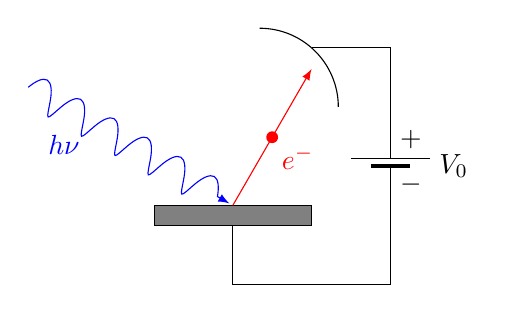
\begin{tikzpicture}
\draw[fill=gray] (0,0) rectangle (2,-.25);
\draw (1,-.25) -- (1,-1) -- (3,-1) --(3,.5) node[anchor=north west]{$-$} node[right=.5cm]{$V_0$};
\draw[very thick] (2.75,.5) -- +(.5,0);
\draw (3,0.6) node[anchor=south west]{$+$} -- (3,2) -- (2,2);
\draw (2.5,.6) -- +(1,0);
\draw (2.34,1.25) arc (0:90:1); 
\draw[red,-latex] (1,0) -- +(60:2);
\fill[red] (1,0) +(60:1) circle (.075cm) node[anchor=north west]{$e^-$};
\draw[decoration={aspect=0.2, segment length=4.9mm, amplitude=2mm,coil},decorate,-latex,blue] (1,0) ++(150:3) -- ++(-30:2.95) node[midway,left=.5cm]{$h\nu$};
\end{tikzpicture}
\end{center}


\begin{center}
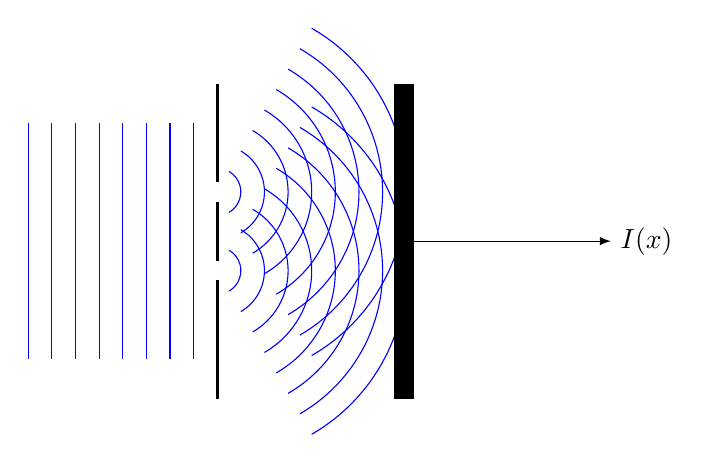
\begin{tikzpicture}
\def\g{.3}
\def\a{60}
\draw[very thick] (0,-.5) -- (0,1) (0,1.25) -- (0,2) (0,2.25) -- (0,3.5);
\foreach\i in {1,...,8} {
    \draw[blue] (-\i * \g,0) -- +(0,3);
    \draw[blue] (0,1.125) +(\a:\i*\g) arc (\a:-\a:\i*\g);
    \draw[blue] (0,2.125) +(\a:\i*\g) arc (\a:-\a:\i*\g);
}

\fill (2.25,-.5) rectangle +(.25,4);

\draw[rotate=-90,yshift=2.5cm,xshift=-1.5cm,domain=-2:2,smooth,red,thick]  plot function{(2-abs(x))*cos(4*x)**2};
\draw[-latex] (2.5,1.5) -- +(2.5,0) node[right]{$I(x)$};
\end{tikzpicture}
\end{center}

\end{document}